% https://pxl-digital.pxl.be/page/seminarie-aarixa-27-02

Het eerste seminaire dat ik volgde voor iTalent ging over Docker, een tool om applicatie in containers te runnen. De spreker Sven Luts, software engineer bij AariXa, gaf uitleg over wat deze tool is, waarom het gebruikt wordt en hoe het achterliggend werkt. Hij maakte ook gebruik van demo's om de aangehaalde onderwerpen te verduidelijken.

In het begin stelde de spreker zich voor. Hij deelde zijn werkplek, zijn hobby's en zijn specialiteiten op gebied van informatica met ons. De introductie van Docker volgde zijn introductie. Docker is een tool gemaakt om het aanmaken, het deployen en het runnen van applicaties in containers te versimpelen.

Vervolgens gaf de spreker een uitleg over waarom je Docker moet gebruiken. Het vereenvoudigt niet alleen het maken en het deployen van software, maar het is ook veel sneller dan een virtuele machine. Het voorkomt de bekende uitspraak: "It works on my machine", dit bekomt Docker door in een afgeschermde en ge"isoleerde omgeving te werken. Deze omgeving bevatten alle benodigde dependencies en requirements. Docker bevat ook een ingebouwd version tracking door gebruik te maken van Docker tags. Een applicatie in een Docker container zal op eender wel systeem exact hetzelfde runnen ongeacht van de reeds ge"installeerde software op het host systeem.

Het volgende onderwerp was een Docker container, wat ze zijn en hoe je er aan kan komen. Een Docker container kan vergeleken worden met een virtuele machine, in de zin dat het ge"isoleerd is van het host systeem en het alle benodigdheden die de applicatie nodig heeft om te runnen. Het verschil met een virtuele machine is dat een Docker container geen operating system moet gaan virtualiseren, wat een virtuele machine wel moet doen. Een Docker container gebruikt het operating system van het host systeem. Hierdoor is een Docker container aanmerkelijk kleiner is formaat dan een virtuele machine en heeft het praktisch geen opstarttijd.

Om een Docker container te bekomen is er eest een image nodig. Aan een Docker image kan je op twee manieren komen: je downloadt het van het internet of je maakt er zelf een. Van een Docker registry kan een Docker image gepulld worden, dit is het equivalent van downloaden van het internet. De image kan ook zelf gebuild worden door het builden van een Dockerfile, een bestand waarin het buildproces van een image gedefinieerd wordt. Een Docker container verkrijg je als je deze Docker image runt. In een Docker container kunnen commits met veranderingen naar de image worden gedaan, waarna je deze Docker image weer naar een registry kan pushen.

De spreker toonde na deze uitleg hoe we Docker zelf konden installeren op ons systeem. Docker werkt achterliggend met Linux en vinden er geen problemen plaats bij een installatie op een Linux systeem. Als de installatie plaats vindt op een Mac of een Windows systeem, gaat er in de achtergrond een virtuele machine met Linux opgestart worden die Docker beheert. Hierop volgde de uitleg van de basis commando's om Docker te beheren en monitoren.

\begin{figure}[!h]
  \centering
  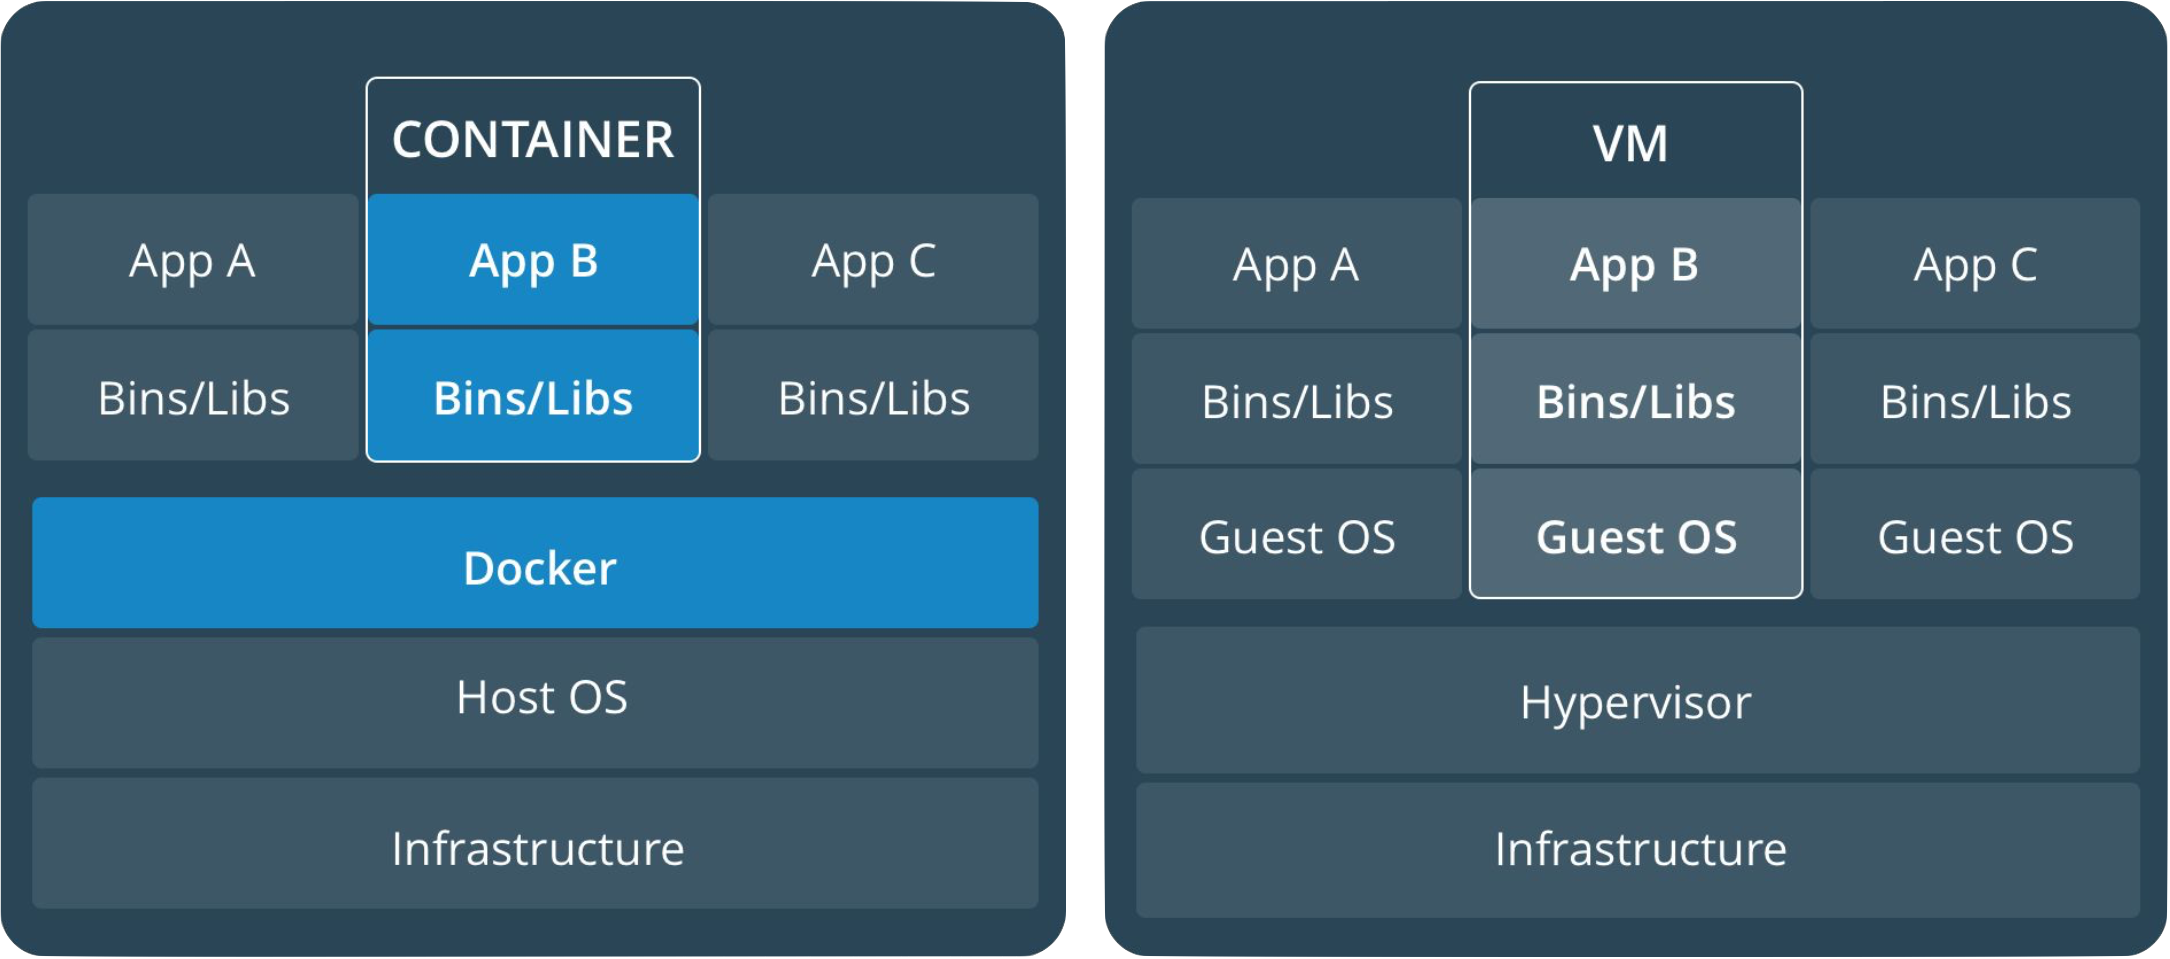
\includegraphics[width=0.72\linewidth]{images/docker/docker_vs_vm.png}
\end{figure}

Het seminarie sloot af met een korte demo over hoe we snel en gemakkelijk Docker commando's konden uittesten in een webapplicatie. Hiervoor moest er dus niets ge"installeerd worden. Deze demo functioneerde als de "Hello World!"\ van Docker. Na de demo gaf de spreker nog een kort vooruitzicht naar wat er in de toekomst met Docker kon gebeuren en gerealiseerd worden.

Het onderwerp van het gegeven seminarie vond ik boeiend, maar ik kon niet plaatsen hoe ik deze technologie zou kunnen gebruiken binnen mijn toekomstige projecten. Echter, toen ik gedurende de vakken rond artifici"ele intelligentie en robotica in aanraking kwam met Docker, zag ik het nut van deze Docker in. Dit gaf mij niet alleen een grote voorsprong op mijn medestudenten die hier nog niet mee in aanraking gekomen waren, maar het deed mij ook beseffen dat het een zeer praktische technologie is waar ik in de toekomst ook nog gebruik van zou maken.

Ondertussen zijn mijn grootste projecten in Docker gemaakt. Namelijk mijn IT\hyp{}project en mijn stage hadden Docker als basis. Het seminarie en de technologie hebben mij ge"inspireerd om ge"isoleerde applicaties te gaan schrijven. Ook ga ik heel anders om met dependencies dan ik voordien deed, ik zorg dat ik altijd een stabiele versie van een bepaalde software gebruik en dat er geen conflicten zijn tussen de gebruikte software. Docker geeft in een bepaalde zin meer vrijheid om te experimenteren met het project. Doordat je altijd terug kan gaan naar een stabiele versie waarin de applicatie werkend is.

De spreker bracht deze presentatie zeer rustig en haalde goede punten aan. Door niet af te dwalen maar toch wat leuke weetjes in zijn presentatie te stoppen, verloor hij niemand zijn aandacht. Hij deelde zijn eigen ervaring met Docker. Zijn projecten konden zonder probleem op elke computer met Docker runnen, zonder dat hij hier enige extra moeiten in had gestoken.

Naar mijn mening is Docker zo handig dat ik het in een laat eerste\hyp{} of vroeg tweedejaarsvak aan zou halen. Dit kan makkelijk in vakken zoals Desktop OS of Server OS Essentials, waar we al kennis maakten met Linux. De tijd die ik al gewonnen heb met Docker en de vrijheid die je er van krijgt, zorgen ervoor dat Docker momenteel een van mijn favoriete en meest gebruikte technologie is.

Spreker: Sven Luts, software engineer bij AariXa, \url{https://be.linkedin.com/in/svenluts/nl}


\begin{figure}[!h]
  \centering
  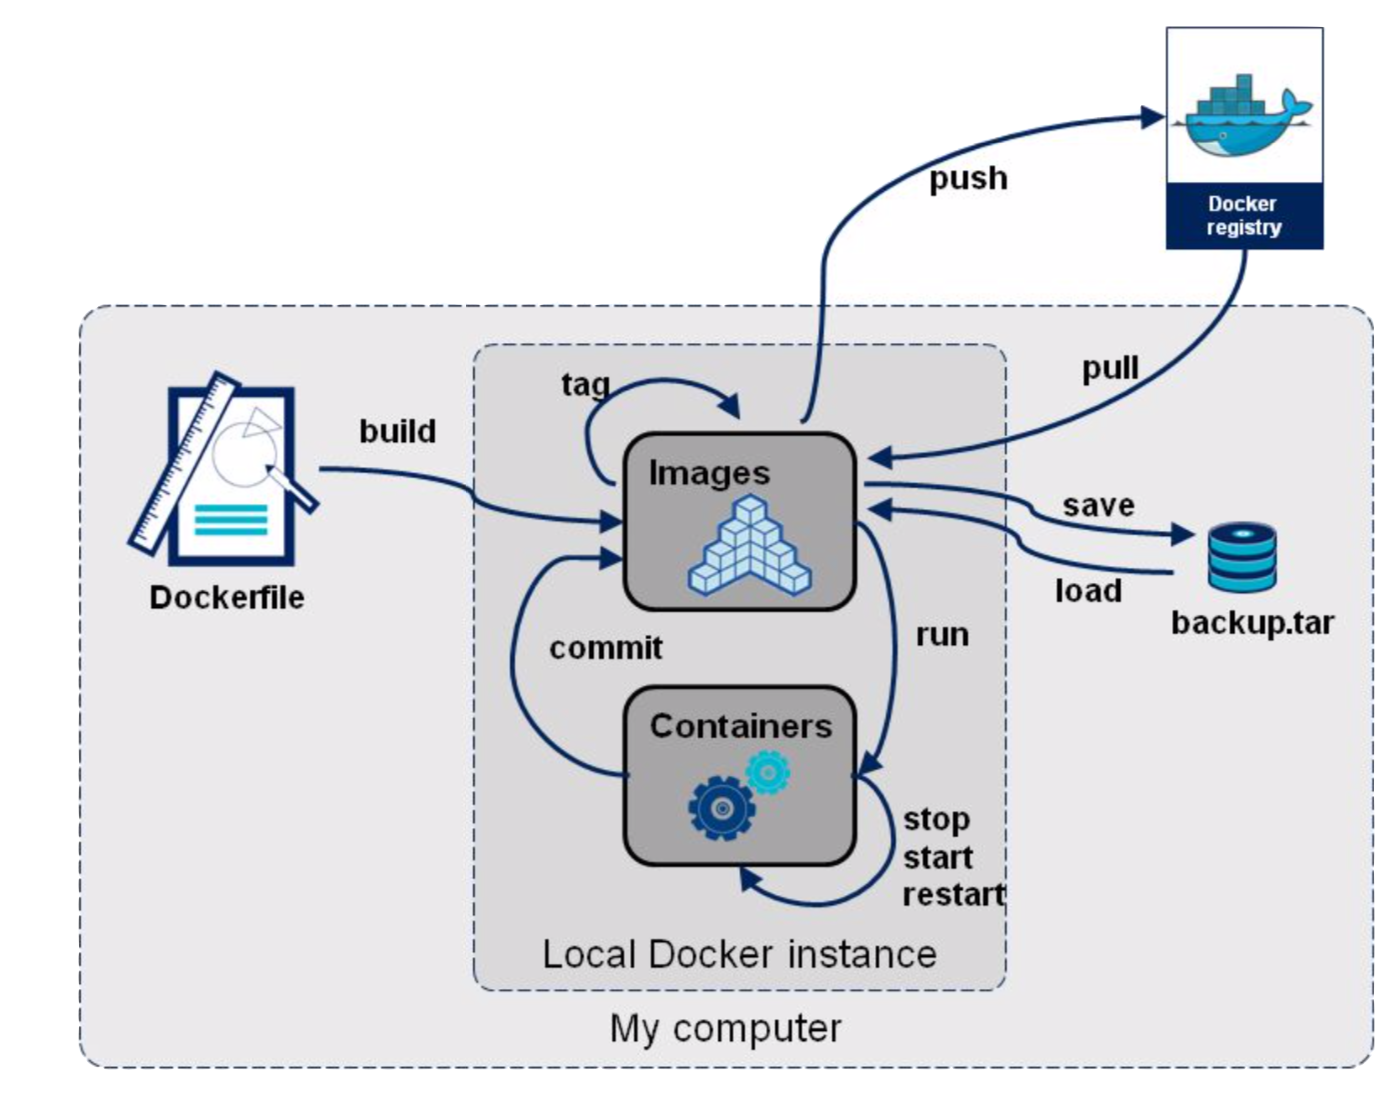
\includegraphics[width=0.74\linewidth]{images/docker/flow.png}
\end{figure}